\section{Algoritmo}
\subsection{Briefing}
Nell'ambito di questa applicazione si considera che ogni piatto sia composto da un ingrediente principale e da più ingredienti secondari. 
Ogni piatto ordinato viene chiamato ordine, quindi un ordine comprende un singolo piatto, mentre la comanda contiene tutti gli ordini di un singolo cliente.
Nel corso di un brainstorming, si è maturata l’idea di organizzare la cucina in postazioni, ognuna focalizzata su un ingrediente principale: ogni postazione si occuperà quindi di preparare e completare piatti accomunati dallo stesso ingrediente principale.
\subsection{Organizzazione} 
Di seguito viene illustrata l’organizzazione delle entità coinvolte nella gestione dell’algoritmo:
\subsubsection{Ordine}
Ogni ordine contiene un singolo piatto del menù, viene classificato per ingrediente principale univoco (es. riso, pasta, pesce, …), ogni ordine presenta poi più parametri, questi contribuiscono a calcolare la priorità ad esso associata.
Parametri ordine:
\begin{itemize}
	\item Ingrediente principale;
	\item Tempo di preparazione;
	\item Numero ordine effettuato (primo, secondo, …);
	\item Urgenza del cliente;
	\item Tempo in attesa.
\end{itemize}

\subsubsection{Cucina}
La cucina viene organizzata in postazioni di lavoro, ossia delle aree dedicate organizzate per svolgere specifiche attività culinarie adibite alla preparazione di piatti che hanno in comune il medesimo ingrediente principale, nello specifico:
\begin{itemize}
	\item ogni postazione di lavoro è adibita al massimo a 1 ingrediente principale;
	\item ogni postazione di lavoro può avere più cuochi (la presenza di più cuochi aumenta la velocità di preparazione della postazione), i cuochi possono spostarsi tra le postazioni;
	\item una postazione può essere vuota, esiste un massimo numero di cuochi per postazione;
	ogni postazione ha una coda di ordini da preparare:
	\begin{itemize}
		\item soglia minima di ordini in coda per poter attivare la postazione;
		\item soglia massima di ordini in coda (oltre la quale si può richiede un cuoco aggiuntivo oppure di rallentare aggiornando il parametro);
		\item tempo massimo in cui gli ordini possono stare in coda di preparazione.
	\end{itemize}
	\item In preparazione possono stare un numero di ordini pari al numero di cuochi;
	\item la somma degli ordini in coda di preparazione è sempre minore della lunghezza della coda di preparazione più piccola.
\end{itemize}

\subsubsection{Postazione}
Con postazione si intende uno spazio di lavoro attrezzato con gli strumenti necessari per lavorare con un particolare tipo di ingrediente principale. Una singola postazione presenta una struttura dati per gestire gli ordini in coda di preparazione, ogni postazione presenta un numero massimo di cuochi che possono lavorare contemporaneamente e può essere attivata solo con un numero minimo di ordini in coda (può essere vuota senza cuochi).
\begin{itemize}
	\item 1 ingrediente principale;
	\item N cuochi (N<M max cuochi per postazione);
	\item 1 struttura dati (coda);
	\item stato (vuota, regolare, intasata).
\end{itemize}

\subsection{Struttura dati}
Per quanto riguarda il flusso di un ordine all’interno del sistema si considera che immediatamente dopo l’ordinazione da parte del cliente viene assegnata una priorità per tale ordine, gli ordini vengono così raccolti nella struttura dati principale con l’etichetta della priorità. Successivamente, se la cucina lo richiede, l'ordine con la priorità più elevata viene spostato nella coda di preparazione della rispettiva postazione di lavoro.

\begin{figure}[htbp]
	\centering
	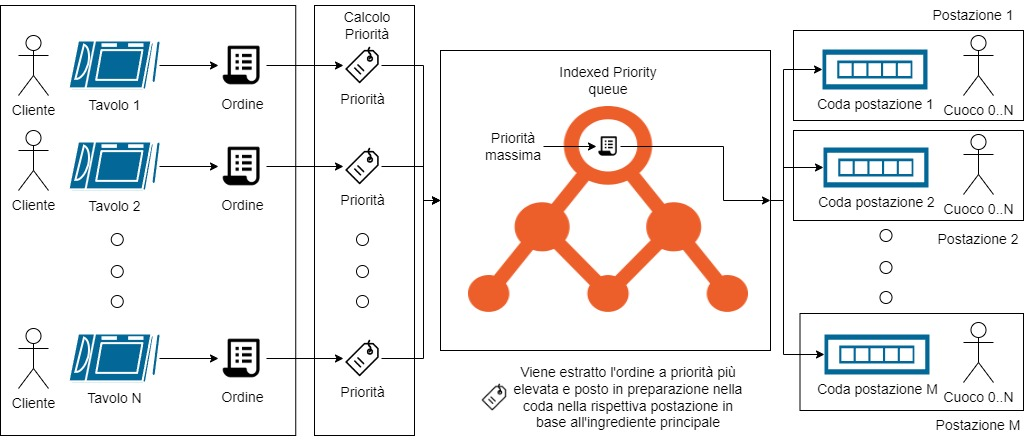
\includegraphics[scale=0.4]{iterazione1/images/Algoritmo_struttura.jpg}
	\caption{Strutture dati dell'algoritmo\label{fig:algoritmo_struttura}}
\end{figure}

Si rendono quindi necessarie due tipi di strutture dati:
\begin{itemize}
	\item Struttura dati principale: Indexed priority queue;
	\item Struttura dati delle postazioni: Coda (queue).
\end{itemize}

\subsection*{Indexed priority queue}
Struttura dati che estende il concetto di coda con priorità aggiungendo la possibilità di accedere in tempo costante agli elementi presenti in coda per compiere operazioni quali la modifica dei parametri, l’aggiornamento della priorità o la rimozione dell’ordine (che altrimenti presenterebbe costo lineare).
Viene implementata per mezzo di una combinazione di una coda con priorità (max heap) e un dizionario (hashtable) che tiene traccia della posizione di ogni elemento all'interno della coda.

\paragraph{Analisi complessità:}
La complessità temporale è correlata a quella di un heap binario, potenziato dall’accesso diretto agli elementi tramite dizionario, di conseguenza:
\begin{itemize}
	\item creazione: O(n);
	\item inserimento e rimozione: O(log n);
	\item modifica priorità: O(log n);
	\item accedere a un elemento: O(1).
\end{itemize}

\paragraph{Requisiti funzionali:}
\begin{itemize}
	\item Gestione degli ordini con priorità: funzionalità chiave della struttura dati, gli ordini ricevono una priorità prima di entrare nella coda a priorità indicizzata;
	\item Fornire l'ordine con priorità più elevata: la struttura dati deve essere in grado di fornire alla cucina l'ordine con la priorità più alta quando richiesto;
	\item Accesso, modifica e rimozione degli ordini: la coda a priorità deve poter fornire la possibilità di implementare la funzionalità che consente ai clienti di accedere, modificare o rimuovere il proprio ordine (nelle prossime iterazioni);
	\item Flessibilità nella modifica delle priorità: la struttura deve garantire una certa flessibilità alla modifica delle priorità degli ordini, poiché le priorità possono cambiare per conto dei clienti, della cucina e a intervalli regolari di tempo.
\end{itemize}

\paragraph{Requisiti non funzionali:}
\begin{itemize}
	\item Tempo di risposta rapido: l’ordine con priorità più elevata deve essere fornito in tempo rapido alla cucina senza ritardi;
	\item Tempo di accesso, modifica e rimozione ragionevole: il cliente deve poter effettuare operazioni senza complicazioni in tempi ragionevoli, mantenendo un’esperienza di utilizzo piacevole;
	\item Scalabilità: La struttura dati deve essere in grado di gestire un grande volume di ordini, adattandosi alle variazioni nella domanda senza compromettere le prestazioni;
	\item Flessibilità alle modifiche: requisito non funzionale relativo alla flessibilità e alla manutenibilità del sistema.
\end{itemize}

\subsection*{Coda (queue)}
Struttura dati lineare che segue il principio "First In, First Out" (FIFO), ossia il principio per il quale il primo elemento che entra nella coda è poi il primo che esce.
\paragraph{Analisi complessità:}
\begin{itemize}
	\item inserimento in coda: O(1);
	\item rimozione della testa: O(1);
	\item verifica stato: O(1) se vuota, O(n) altrimenti.
\end{itemize}

\paragraph{Requisiti funzionali:}
\begin{itemize}
	\item Funzionamento FIFO: La coda deve garantire il corretto funzionamento FIFO (First In, First Out), indipendentemente dalle priorità degli ordini;
	\item Soglia di attivazione: Il sistema deve permettere di configurare una soglia di valore minimo di attivazione per la coda, al di sotto della quale la postazione non viene attivata;
	\item Soglia critica di intasamento: Il sistema deve permettere di configurare una soglia di valore critico, oltre la quale la postazione diventa intasata e richiede operazioni per ridurre il carico.
\end{itemize}

\paragraph{Requisiti non funzionali:}
\begin{itemize}
	\item Lunghezza finita della coda: Il sistema deve gestire una coda con una lunghezza finita, limitata dalla capacità della postazione di lavoro;
	\item Tempo massimo di attesa in coda: Il sistema deve garantire che gli ordini non rimangano in coda di preparazione per troppo tempo prima di essere elaborati;
	\item Attivazione anticipata della postazione: In casi di eccessivo ritardo nella preparazione degli ordini, il sistema può attivare una postazione di lavoro anche se è al di sotto della soglia minima di attivazione.
\end{itemize}

\subsection{Funzione di priorità}
La funzione di priorità è una funzione matematica che assegna un valore numerico decimale di priorità nell’intervallo tra 0 e 1 basandosi sui parametri specifici di ogni ordine.
Il primo passo consiste nel processo di normalizzazione dei parametri, il quale permette di standardizzare i valori in modo che siano compresi tra 0 e 1. in maniera tale da mettere i diversi parametri su una scala comune e uniforme

\subsection*{Parametri}

\paragraph{x1 ingrediente principale:}
Indica il valore di priorità che presenta l'ingrediente predominante dell’ordine, questo valore è influenzato direttamente dallo stato della postazione di lavoro associata in cucina.
\begin{itemize}	
	\item condizione iniziale ogni ingrediente ha valore 0.5
	\item se la cucina è satura ridurre il valore (min 0)
	\item se la cucina è scarica aumentare il valore (max 1)
\end{itemize}

\paragraph{x2 tempo di preparazione:}
Rappresenta la durata stimata necessaria per preparare un determinato ordine.
\begin{itemize}	
	\item normalizzazione: \begin{equation*}
 		\text{tp}_{\text{norm}} = \frac{\text{tp} - \text{tp}_{\text{min}}}{\text{tp}_{\text{max}} - \text{tp}_{\text{min}}}
 	\end{equation*} con tp: tempo di preparazione,\\
 	$\text{tp}_{\text{max}}: \text{tempo di preparazione massimo,}$\\
 	$\text{tp}_{\text{min}}: \text{tempo di preparazione minimo;}$	
	\item $\text{considerare x2 = tp}_{\text{norm}} \text{ per prioritizzare ordini più lunghi,}\\ \text{oppure x2 = 1-tp}_{\text{norm}} \text{ per prioritizzare ordini più brevi.}$
\end{itemize}

\paragraph{x3 urgenza del cliente:}
Consente ai clienti di specificare la tempestività con cui desiderano ricevere il proprio ordine, in particolare i clienti possono chiedere espressamente di avere urgenza, al contrario possono specificare di non avere fretta o non dire nulla e tenere un valore di urgenza di default
\begin{itemize}
	\item 1 se il cliente ha espresso urgenza;
	\item 0 se ha espresso di ritardare o fare con calma;
	\item valore neutro standard 0.5.
\end{itemize}

\paragraph{x4 numero ordine effettuato:}
Specifica il numero dell’ordine del cliente in ordine temporale, in particolare indica la posizione relativa di un ordine all'interno della sequenza di ordini effettuati.
\begin{itemize}
	\item il primo ordine effettuato ha priorità maggiore, mentre i successivi hanno priorità decrescente;
	\item normalizzazione: \begin{equation*}
		\text{x4} = \frac{\text{noe} - 1}{\text{max}_{\text{noe}} - 1}
	\end{equation*} con noe: numero ordini effettuati,\\
	$\text{max}_{\text{noe}} \text{: massimo numero ordini effettuabili;}$
	\item considerare un valore massimo di ordini (es.5 gli ordini dopo il quinto sono comunque consentiti e prenderanno la stessa priorità del 5° ordine).
\end{itemize}

\paragraph{x5 tempo in attesa:}
Rappresenta il periodo di tempo trascorso da quando un ordine è stato effettuato fino al momento in cui viene elaborato.
\begin{itemize}
	\item normalizzazione: \begin{equation*}
		\text{x5} = \frac{\text{tempo in attesa}}{\text{tempo max in attesa}}
	\end{equation*}
	\item considerare un valore massimo di tempo in attesa consentito, in prossimità del quale si ha la priorità più elevata.
\end{itemize}

\subsection*{Pesi}
I pesi sono utilizzati per attribuire un grado di importanza relativo a ciascun parametro all'interno della funzione di priorità. Questi pesi indicano quanto ciascun parametro dovrebbe influenzare il calcolo complessivo della priorità di un determinato elemento.
Si elencano di seguito i pesi per ciascun parametro definito poc’anzi:
\begin{itemize}
	\item p1: peso ingrediente principale;
	\item p2: peso tempo di preparazione;
	\item p3: peso urgenza cliente;
	\item p4: peso numero ordine;
	\item p5: peso tempo in attesa.
\end{itemize}

Viene quindi fatto un ragionamento sull’importanza da attribuire a ogni parametro tramite l’incidenza assegnata al singolo peso. Si dividono quindi i pesi in tre categorie.

\paragraph{Maggiore incidenza} I pesi che devono essere più incidenti sono:
\begin{itemize}
	\item p1 peso ingrediente principale: per evitare di sovraccaricare una postazione rispetto alle altre o per non avere postazioni vuote;
	\item p5 peso tempo in attesa: un ordine non può restare in attesa troppo a lungo.
\end{itemize}

\paragraph{Incidenza media} Il peso con incidenza media è:
\begin{itemize}
	\item p3 peso urgenza del cliente: è meno importante dei vincoli di sovraccarico e attesa, ma deve essere comunque una scelta significativa.
\end{itemize}

\paragraph{Bassa incidenza} I pesi con bassa incidenza sulla priorità sono:
\begin{itemize}
	\item p2 peso tempo di preparazione: in confronto ad altri parametri con pesi più elevati, questo è considerato meno critico;
	\item p4 peso numero ordine effettuato: ha un impatto di poco conto sulla priorità dell’ordine.
\end{itemize}

\subsubsection*{Valore dei pesi}
I valori dei pesi vengono quindi definiti inizialmente:
\begin{itemize}
	\item p1 = 0.25;
	\item p2 = 0.15;
	\item p3 = 0.20;
	\item p4 = 0.15;
	\item p5 = 0.25.
\end{itemize}
Questi valori possono essere regolati col tempo per aumentare l’efficienza dell’algoritmo, diventa così importante raccogliere dati storici per poterli analizzare e comprendere come i vari parametri influenzano le prestazioni del sistema, oltre a raccogliere feedback dei clienti, sulla base di ciò sarà richiesto un tuning dei pesi più accurato. Per questo motivo è richiesta una certa flessibilità in modo da consentire l'aggiornamento dei pesi dei parametri in modo dinamico.

\subsection*{Funzione matematica}
L'equazione proposta rappresenta una somma pesata dei parametri, dove ciascun parametro (x1, x2, x3, x4, x5) viene moltiplicato per il suo relativo peso (p1, p2, p3, p4, p5). I pesi indicano l'importanza relativa dei parametri nel determinare la priorità complessiva di un elemento. La somma pesata dei parametri produce un valore (y) compreso tra 0 e 1, dove 0 indica un valore meno urgente e 1 indica un valore più urgente.
\begin{equation*}
	\text{y} = \text{p1}*{\text{x1}} + \text{p2}*{\text{x2}}  + \text{p3}*{\text{x3}}  + \text{p4}*{\text{x4}}  + \text{p5}*{\text{x5}} 
\end{equation*}

\subsection{Diagramma di flusso}
Per comprendere meglio il processo dell’algoritmo viene mostrato il diagramma di flusso in \figurename~\ref{fig:flowchart}, nel quale viene mostrato il flusso di un ordine dal momento in cui viene effettuato dal cliente a quando viene assegnato alla postazione di lavoro in cucina.
\begin{figure}[htbp]
	\centering
	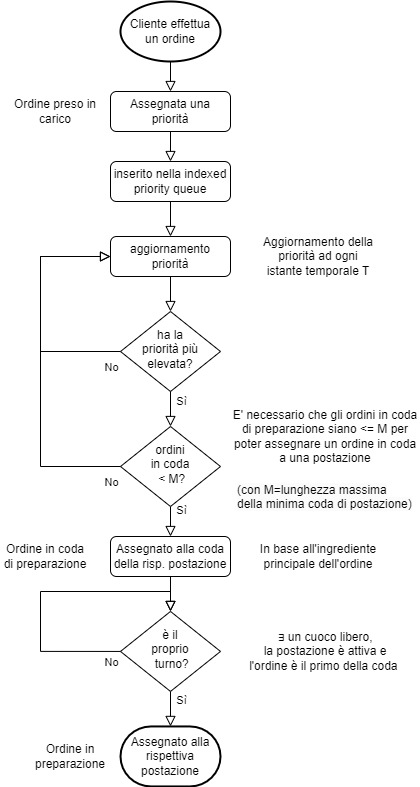
\includegraphics[scale=0.7]{iterazione1/images/flowchart.jpg}
	\caption{Diagramma di flusso\label{fig:flowchart}}
\end{figure}